% Pipeline figure for the paper (one IEEE column, 3.5 in wide, no title).
% Compile from the project root:
%   mkdir -p plots/out/pipeline
%   pdflatex -interaction=nonstopmode -jobname=pipeline \
%            -output-directory=plots/out/pipeline plots/scripts/fig_pipeline.tex
% -> plots/out/pipeline/pipeline.pdf (the .aux and .log land next to it).
%
% Colours are the paper palette (plots/paper_labels.py): boxes = COLORS["core"]
% (#0072B2), zones = COLORS["band"] (#E6E6E6). Times via mathptmx, all text 8 pt.
% Layout (y grows downwards, inches): left column = main flow, right column =
% side branch (Distribution analysis); the "language" arrow runs down the
% left margin (x = -1.6 in), left of the boxes and of the zone labels, so it
% crosses neither text nor boxes. Subtitles are italic.
\documentclass[border=0.5pt]{standalone}
\usepackage[T1]{fontenc}
\usepackage{mathptmx}
\usepackage{tikz}
\usetikzlibrary{arrows.meta}

\definecolor{boxblue}{HTML}{0072B2}
\definecolor{zonegray}{HTML}{E6E6E6}
\definecolor{zoneedge}{HTML}{999999}

\newcommand{\pfs}{\fontsize{8}{9.6}\selectfont}

\begin{document}
\frenchspacing % no extra space after ":" and ";"
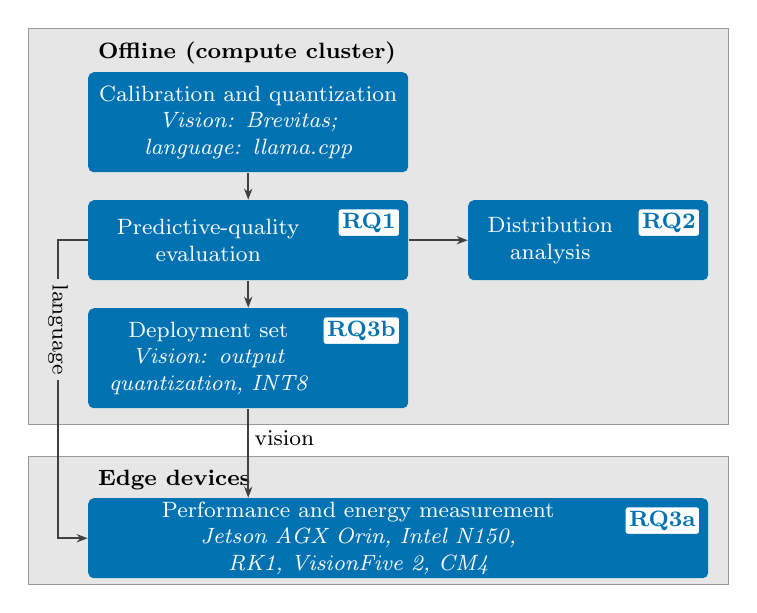
\begin{tikzpicture}[
  font=\pfs,
  boxrect/.style={rectangle, rounded corners=2pt, fill=boxblue, inner sep=0pt},
  boxtext/.style={text=white, align=center, inner sep=0pt},
  tag/.style={rectangle, rounded corners=1pt, draw=boxblue, line width=0.5pt, fill=white,
              text=boxblue, inner sep=1.5pt, font=\pfs\bfseries, anchor=north east},
  zlabel/.style={anchor=north west, font=\pfs\bfseries, text=black},
  flow/.style={-{Stealth[length=4pt, width=3pt]}, line width=0.6pt, draw=black!75},
  elabel/.style={font=\pfs, text=black, inner sep=2pt},
]

% zones (drawn first so boxes and arrows sit on top)
\fill[zonegray, draw=zoneedge, line width=0.4pt] (-1.75in, 0in) rectangle (1.75in, -1.98in);
\fill[zonegray, draw=zoneedge, line width=0.4pt] (-1.75in, -2.14in) rectangle (1.75in, -2.78in);
\node[zlabel] at (-1.45in, -0.02in) {Offline (compute cluster)};
\node[zlabel] at (-1.45in, -2.16in) {Edge devices};

% boxes: main column x in [-1.45, 0.15] in, side column x in [0.45, 1.65] in
\node[boxrect, minimum width=1.6in, minimum height=0.5in] (b1) at (-0.65in, -0.47in) {};
\node[boxtext, text width=1.52in] at (b1.center)
  {Calibration and quantization\\ {\itshape Vision: Brevitas;\\ language: llama.cpp}};

\node[boxrect, minimum width=1.6in, minimum height=0.4in] (b2) at (-0.65in, -1.06in) {};
\node[boxtext, text width=1.2in] at ([xshift=-0.2in]b2.center) {Predictive-quality\\ evaluation};
\node[tag] at ([shift={(-3pt,-3pt)}]b2.north east) {RQ1};

\node[boxrect, minimum width=1.2in, minimum height=0.4in] (b3) at (1.05in, -1.06in) {};
\node[boxtext, text width=0.82in] at ([xshift=-0.19in]b3.center) {Distribution analysis};
\node[tag] at ([shift={(-3pt,-3pt)}]b3.north east) {RQ2};

\node[boxrect, minimum width=1.6in, minimum height=0.5in] (b4) at (-0.65in, -1.65in) {};
\node[boxtext, text width=1.2in] at ([xshift=-0.2in]b4.center)
  {Deployment set\\ {\itshape Vision: output\\ quantization, INT8}};
\node[tag] at ([shift={(-3pt,-3pt)}]b4.north east) {RQ3b};

\node[boxrect, minimum width=3.1in, minimum height=0.4in] (b5) at (0.1in, -2.55in) {};
\node[boxtext, text width=2.65in] at ([xshift=-0.2in]b5.center)
  {Performance and energy measurement\\ {\itshape Jetson AGX Orin, Intel N150, RK1, VisionFive 2, CM4}};
\node[tag] at ([shift={(-3pt,-3pt)}]b5.north east) {RQ3a};

% flow
\draw[flow] (b1.south) -- (b2.north);
\draw[flow] (b2.south) -- (b4.north);
\draw[flow] (b2.east) -- (b3.west);
\draw[flow] (b4.south) -- node[elabel, pos=0.33, right] {vision} (b4.south |- b5.north);
\draw[flow] (b2.west) -- (-1.6in, -1.06in) --
  node[elabel, pos=0.3, sloped, fill=zonegray] {language} (-1.6in, -2.55in) -- (b5.west);
\end{tikzpicture}
\end{document}
